%************************************************
\chapter{Spatial distribution of the Southern Ocean carbon sink}\label{ch:spatial} % $\mathbb{ZNR}$
%************************************************
\section{Spatial internal variability}

The large ensemble median represents the forced signal and the standard deviation represents internal variability \citep{Deser2012}. The forced signal shows a dominant increasing trend in the Southern Ocean carbon sink (Fig. \ref{fig:SOCS_ensmean_ensstd} top left). Also in spatial distribution, the carbon sink in each grid point follows a normal distribution (Fig. SI \ref{fig:SOCS_temporal_gaussian}). The standard deviation (Fig. \ref{fig:SOCS_ensmean_ensstd} top right) shows differences in magnitude of internal variability in a zonal pattern. The largest internal variability appears in 50-60$^\circ$S south of the polar front. Internal variability drops north of 45$^\circ$S, showing the large internal variability of the Southern Ocean compared to other ocean basins.


\begin{figure}[h]
\centering
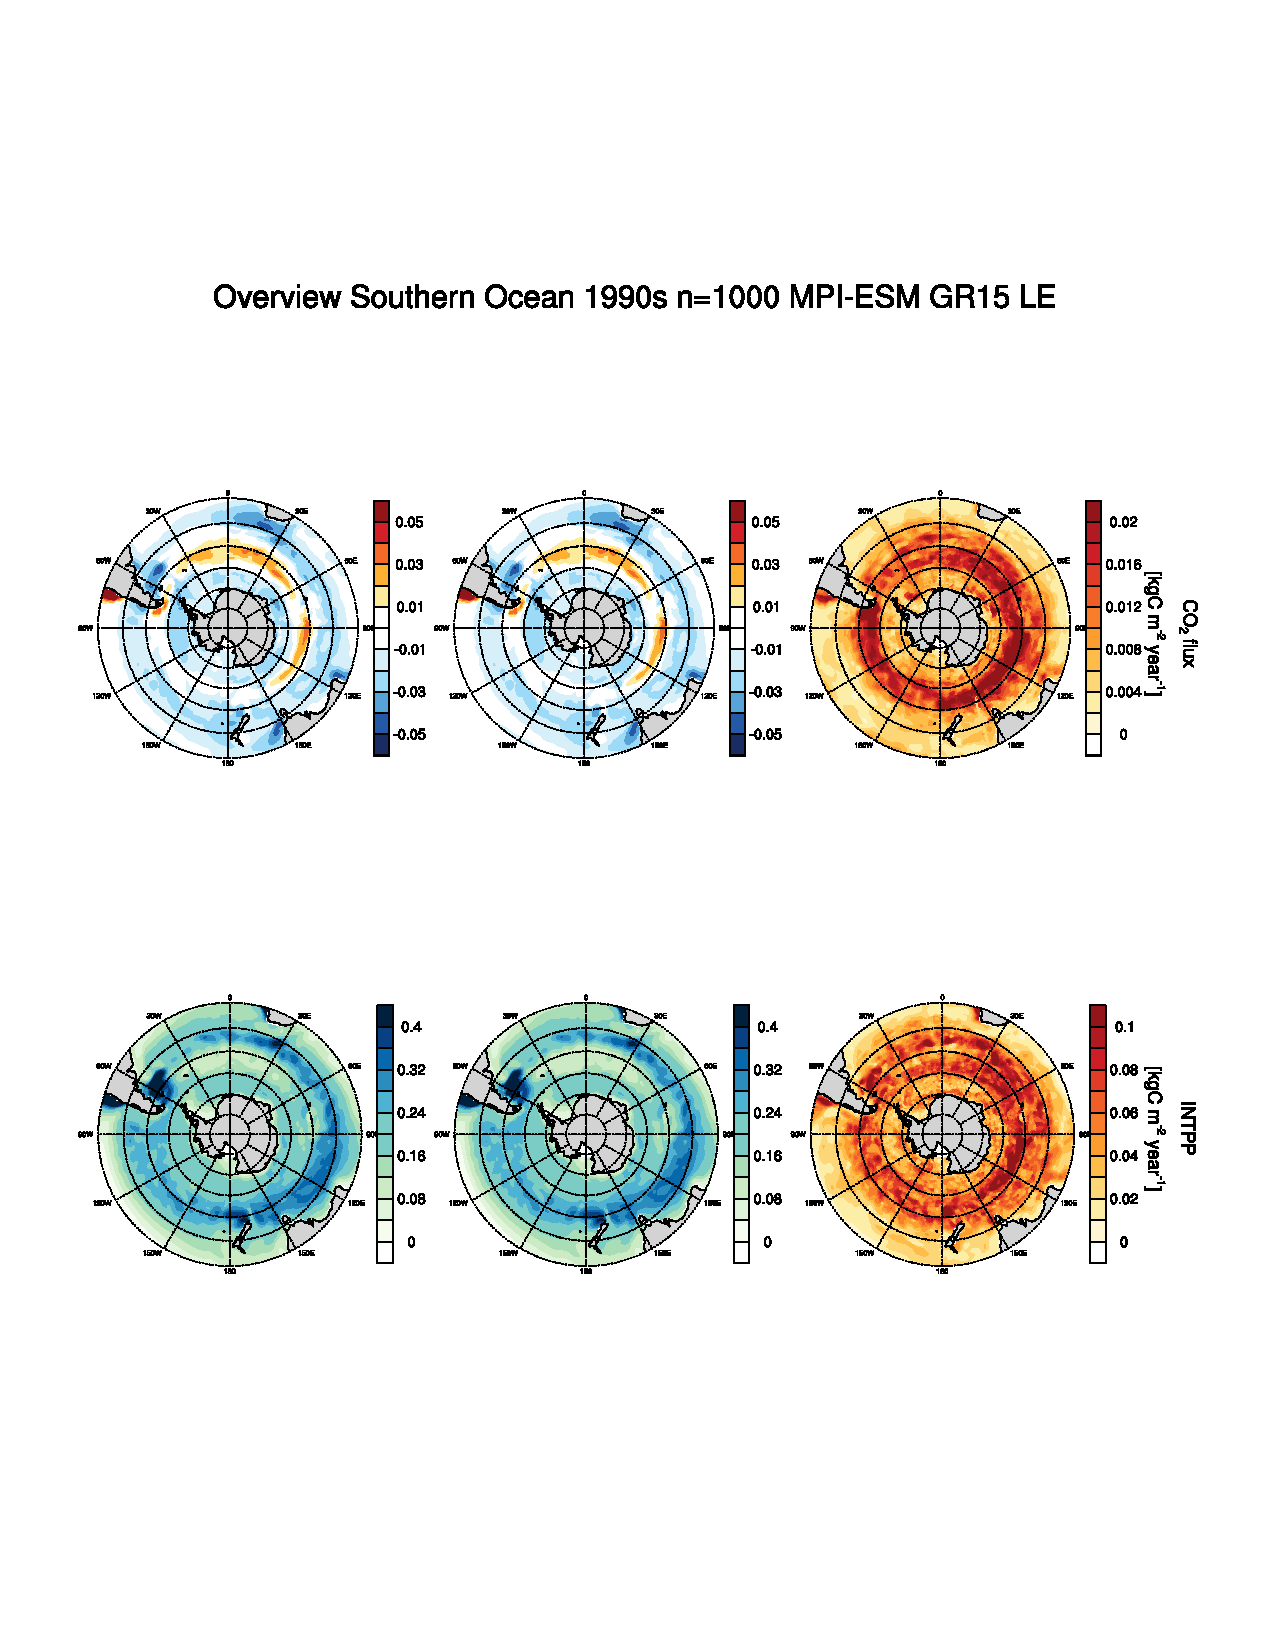
\includegraphics[scale=.9,trim=7.2cm 15cm 0cm 8cm,clip]{gfx/Overview_SO_co2flux_intpp_ens_t1990s.pdf} % from gfx folder
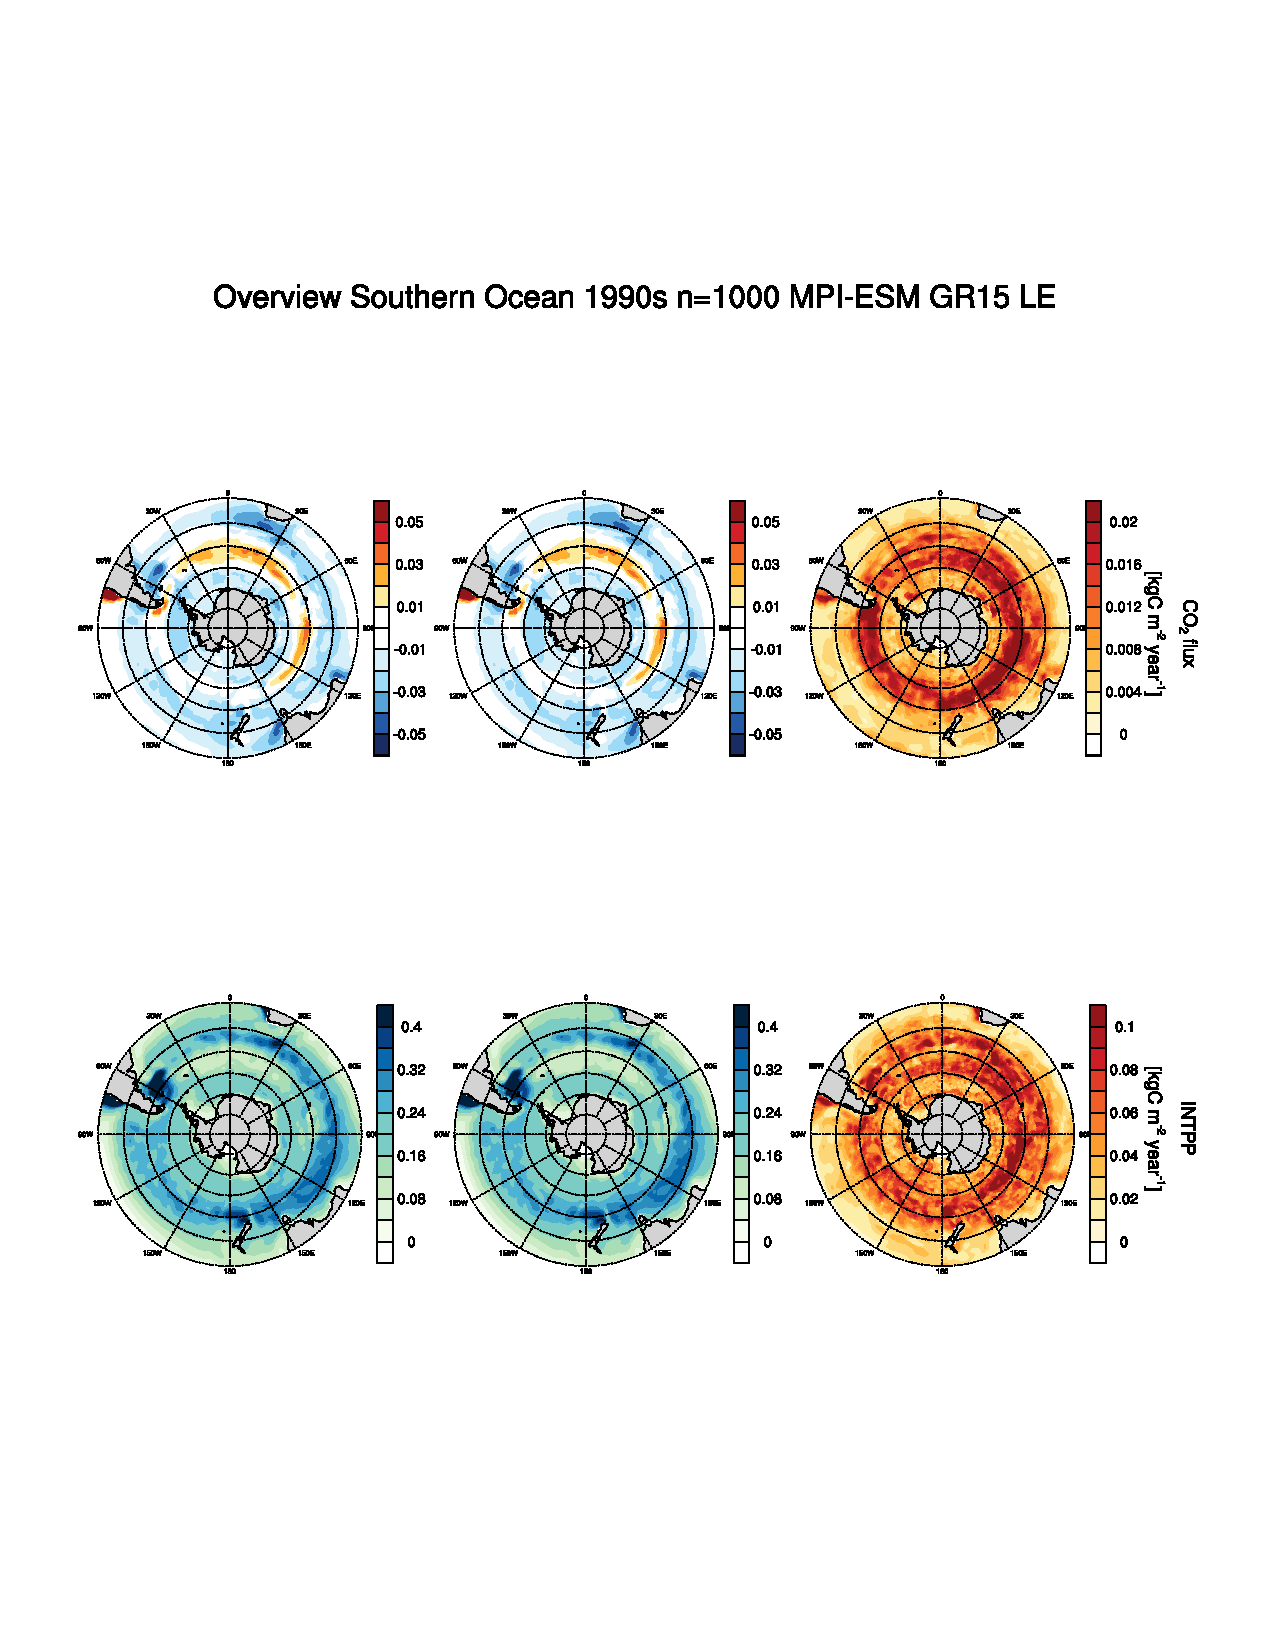
\includegraphics[scale=.9,trim=7.2cm 6.3cm 0cm 16cm,clip]{gfx/Overview_SO_co2flux_intpp_ens_t1990s.pdf} % from gfx folder
\caption{Southern Ocean CO$_2$flux where negative values indicate ocean uptake (top) and primary production (bottom): ensemble median (left) as forced signal and ensemble standard deviation (right) as internal variability}
\label{fig:SOCS_ensmean_ensstd}
\end{figure}




\section{Negative trend of the Southern Ocean carbon sink}

\begin{figure}[h]
\includegraphics[scale=1.,trim=13.25cm 18.7cm 2.5cm 6cm,clip]{gfx/\member _positive_trend_8_obgc_overview_summer.pdf} %co2flux
\includegraphics[scale=1.,trim=13.25cm 15.9cm 2.5cm 9.2cm,clip]{gfx/\member _positive_trend_8_obgc_overview_summer.pdf} %intpp
\includegraphics[scale=1.,trim=13.25cm 13.1cm 2.5cm 12.1cm,clip]{gfx/\member _positive_trend_8_obgc_overview_summer.pdf} %nutlimf
\includegraphics[scale=1.,trim=13.25cm 7.3cm 2.5cm 17.8cm,clip]{gfx/\member _positive_trend_8_obgc_overview_summer.pdf} %zmld
\caption{Southern Ocean austral summer trends per per 8 years: CO$_2$flux (top left), vertically integrated primary production (top right), nutrient limitation (bottom right) and mixed layer depth (bottom left); hatched areas indicate where trends were below 5\% significance}
\label{fig:co2flux_intpp}
\end{figure}

\begin{figure}[h]
%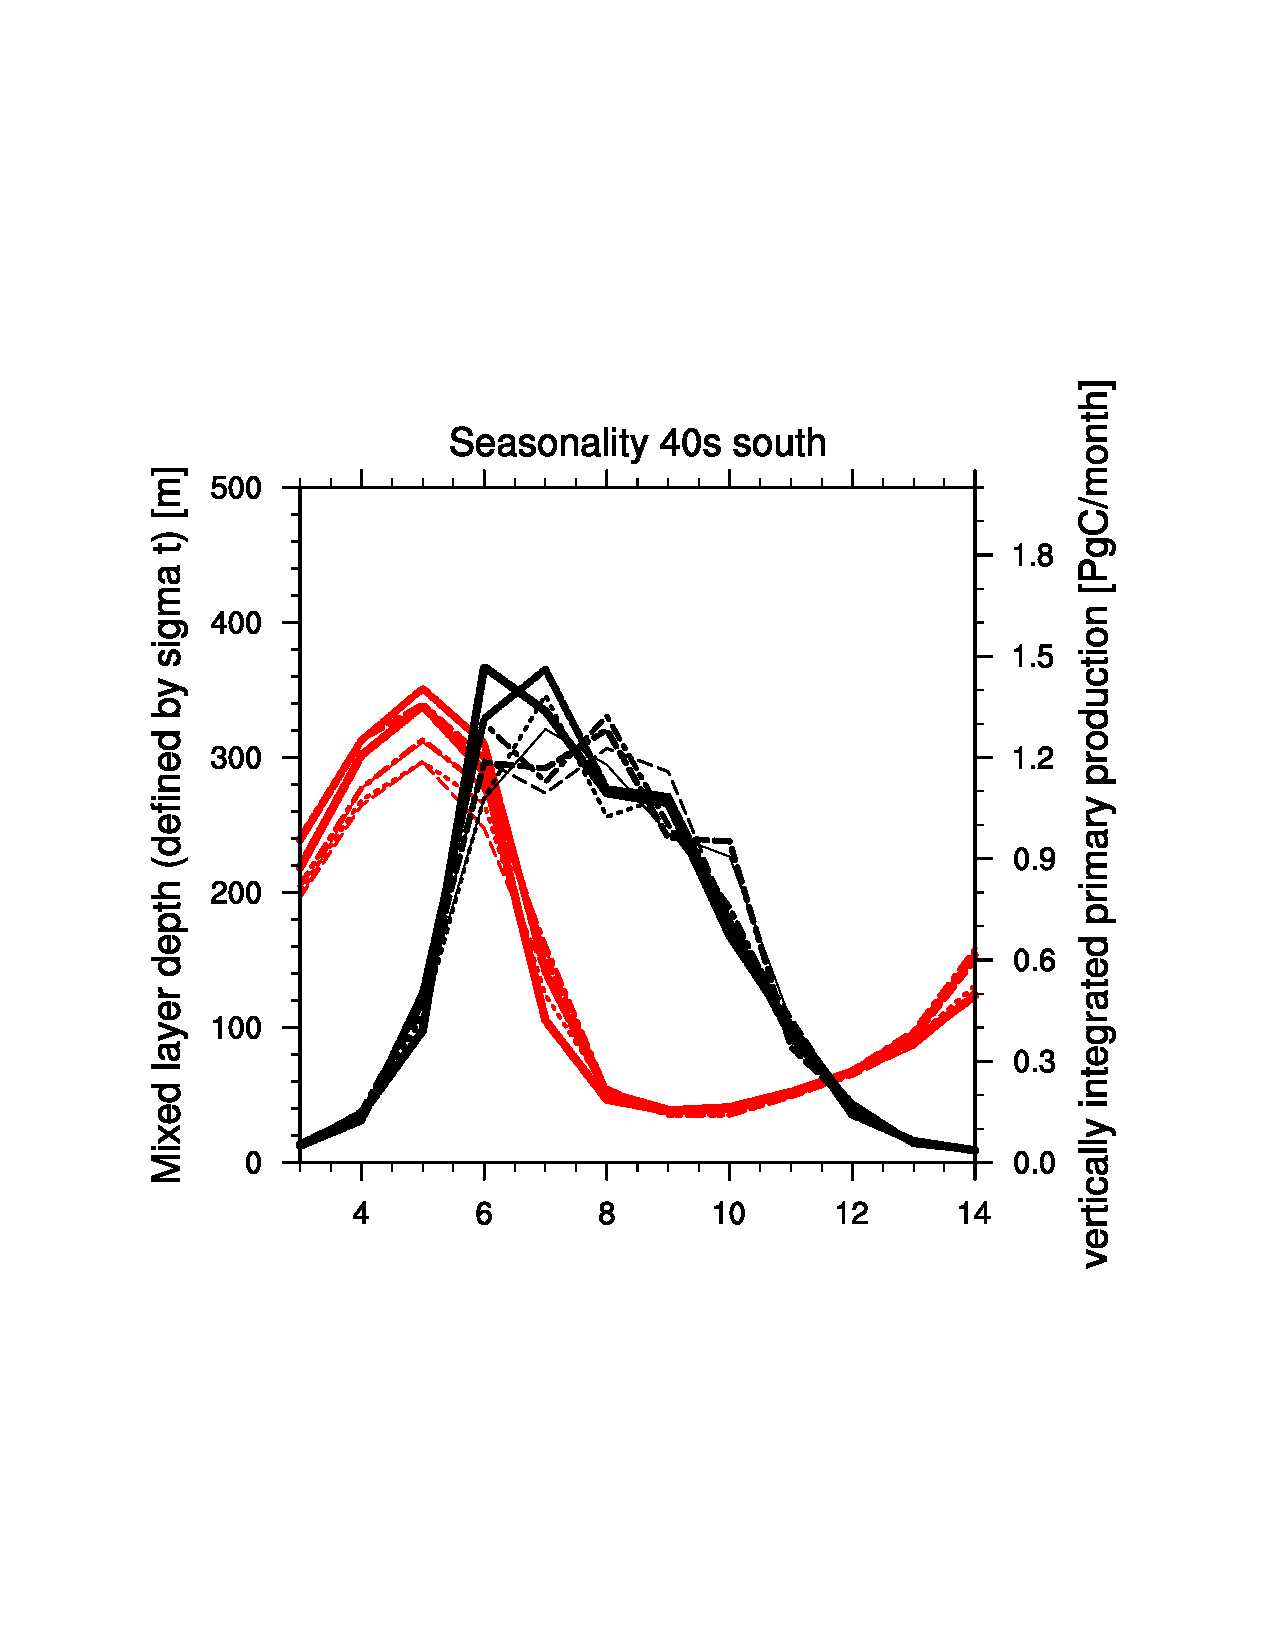
\includegraphics[scale=.4,trim=0cm 6cm 0cm 5cm,clip]{seasonality_intpp_zmld_area40} % from gfx folder
\centering
\includegraphics[page=2,scale=.6,trim=0cm 6cm 0cm 5cm,clip]{gfx/\member _positive_trend_8_seasonality_intpp_zmld.pdf} % from gfx folder
%\vspace{-1cm}
\caption{Seasonality of vertically integrated primary production (black) and mixed layer depth (red) at 50-60$^\circ$S over 8 years; thicker lines are later years}
\label{fig:zmld_intpp_seasonality}
\end{figure}

\begin{figure}
\includegraphics[scale=.65,trim=1.2cm 13.2cm 0cm 7cm,clip]{gfx/\member _positive_trend_8_schwerpunkt_mixing_overview.pdf}
\caption{Trends in [m/8yrs] for phytoplankton average depth (left) and average depth of vertical diffusivity due to wind (right); hatched areas indicate where trends were below 5\% significance}
\label{fig:wind_mixing}
\end{figure}

\section{Positive trend of the Southern Ocean carbon sink}


